%%%%%%%%%%%%%%%%%%%%%%%%%%%%%%%%%%%%%%%%%%%%%%%%%%%%%%%
%
% chapter02 - Behavioral Types
%
%%%%%%%%%%%%%%%%%%%%%%%%%%%%%%%%%%%%%%%%%%%%%%%%%%%%%%%

%
% >>>>>>>>>>>>>>> PLEASE NOTE <<<<<<<<<<<<<<<
%
% This file is not stand-alone compileable as it is, to make it compileable while writing uncomment the preamble below.
% In this case, you also have to uncomment the begin/end document statements.
% You can outcomment the preamble and the begin/end document statements again or erase them when handing in your contribution.
%
% If you use BibTex for your bibliography, please use \putbib[bibliography] to print your reference (see end of this file).
%
% you can use paths relative to your chapter dir, e.g. \figure{assets/fig1}.
%
% >>>>>>>>>>>>>>>>>>>><<<<<<<<<<<<<<<<<<<<<<<

%%%%%%%%%%%%%%%%%%%%%%%%%%%%%%%%%%%%%%%%%%%%%%%%%%
%% you can uncomment the following preamble during development to make this file compileable.
%% Note that you need the svmult.cs file inside your chapter root dir to make this work.
%% Also note that if you need additional packages etc., you can add them here, but please
%% mark them somehow so the editor of this book knows you need them in the final book.
%% When you hand in your contribution, please uncomment or remove the preamble again.
%%%%%%%%%%%%%%%%%%%%%%%%%%%%%%%%%%%%%%%%%%%%%%%%%%
%%%%%%%%%%%%%%%%%%%%%%%%%%%%%%%%%%%%%%%%%%%%%%%%%%% start of preamble
\documentclass[
graybox,
envcountchap
]{svmult}

\usepackage[utf8]{inputenc}
\usepackage{mathpartir}
%\usepackage{type1cm}        % activate if the above 3 fonts are
% not available on your system

\usepackage{makeidx}         % allows index generation
\usepackage{graphicx}        % standard LaTeX graphics tool
% when including figure files
\usepackage{multicol}        % used for the two-column index
\usepackage[bottom]{footmisc}% places footnotes at page bottom
\usepackage{url}
\usepackage{newtxtext}       %
\usepackage{newtxmath}       % selects Times Roman as basic font

% \usepackage{natbib}
\usepackage{footmisc}

%% Additional packages added. Add necessary packages here.
%\usepackage[english]{babel}
\usepackage{siunitx}
\usepackage{amssymb}
\usepackage{pifont}
\usepackage{xcolor}
\usepackage{tabularx}
\usepackage{listings}
\usepackage{booktabs}
\usepackage{hyperref}
\usepackage{url}
\usepackage{mathtools}
\usepackage{lipsum}
\usepackage{import}
\usepackage{bibunits}
\usepackage{acronym}
\usepackage[nottoc]{tocbibind}
\usepackage{numberpt}
\usepackage{stmaryrd}
\usepackage{amsmath}

\usepackage{listings}
\usepackage{upquote}
\usepackage{color}

\definecolor{bluekeywords}{rgb}{0.13,0.13,1}
\definecolor{greencomments}{rgb}{0,0.5,0}
\definecolor{turqusnumbers}{rgb}{0.17,0.57,0.69}
\definecolor{redstrings}{rgb}{0.5,0,0}

\lstdefinelanguage{scribble}{
  morekeywords={
  	global, protocol, role, from, to, interruptible, with, do, instantiates, par, and, rec, continue, choice, at, initiates, handle, returning, call, local, or, self
  },
  otherkeywords={ },
  keywordstyle=\color{bluekeywords},
  sensitive=true,
  %basicstyle=\scriptsize\ttfamily,
  basicstyle=\linespread{0.9}\ttfamily,
	breaklines=true,
  xleftmargin=\parindent,
  belowskip=\bigskipamount,
  aboveskip=\bigskipamount,
  tabsize=4,
  morecomment=[l][\color{greencomments}]{///},
  morecomment=[l][\color{greencomments}]{//},
  morecomment=[s][\color{greencomments}]{{(*}{*)}},
  morestring=[b]",
  showstringspaces=false,
  literate={`}{\`}1,
  frame=none,
  showlines=false,
  %frame=single,
  stringstyle=\color{redstrings},
}



\newcommand{\todo}[1]{{\noindent\small\color{red} \framebox{\parbox{\dimexpr\linewidth-2\fboxsep-2\fboxrule}{\textbf{TODO:} #1}}}}

\newcommand*{\CHAPTERSROOT}{../.}	% root path for chapters.
\newcommand*{\chapterprefix}{02}	% your chapter number.

\newcommand{\mkwd}[1]{\ensuremath{\mathsf{#1}}}
\usepackage{subfig}
\usepackage{tikz}
\usetikzlibrary{matrix,fit}
\usepackage[scaled]{beramono}
\usepackage[T1]{fontenc}
\usepackage{listings}
\lstset{
  basicstyle=\ttfamily
}

\newcommand{\mypar}[1]{\vspace{1em}\textbf{#1}\quad}

\newcommand{\calcwd}[1]{\textbf{\textsf{#1}}}
\newcommand{\actsend}[2]{\calcwd{send} :\ #1 \: #2}
\newcommand{\pid}[1]{\mkwd{ActorRef}(#1)}
\newcommand{\seq}[1]{\overrightarrow{#1}}
\newcommand{\totheleft}[1]{\begin{flushleft}#1\end{flushleft}}

\newcommand{\chan}[1]{\mkwd{Chan}(#1)}
\newcommand{\var}[1]{\mathit{#1}}
\newcommand{\newch}{\calcwd{newCh}}
\newcommand{\gvsend}[2]{\calcwd{send} \: #1 \: #2}
\newcommand{\gvrecv}[1]{\calcwd{receive} \: #1}
\newcommand{\gvclose}[1]{\calcwd{close} \: #1}
\newcommand{\letintwo}[2]{\calcwd{let} \: #1 = #2 \: \calcwd{in}}
\newcommand{\bl}{\begin{array}{l}}
\newcommand{\blt}{\begin{array}[t]{l}}
\newcommand{\el}{\end{array}}
\newcommand{\defeq}{\triangleq}
\newcommand{\metadef}{\mkwd}
\newcommand{\lto}{\multimap}
\newcommand{\one}{\mathbf{1}}
\newcommand{\gvdual}[1]{\overline{#1}}
\newcommand{\gvend}{\mkwd{End}}
\newcommand{\gvout}[2]{{!}#1{.}#2}
\newcommand{\gvin}[2]{{?}#1{.}#2}

\newcommand{\triestosend}[4]{{#1} \xRightarrow[#4]{#2} {#3}}
\newcommand{\intty}{\mkwd{Int}}
\newcommand{\boolty}{\mkwd{Bool}}
\newcommand{\stringty}{\mkwd{String}}

\makeindex % used for the subject index
%%%%%%%%%%%%%%%%%%%%%%%%%%%%%%%%%%%%%%%%%%%%%% end of preamble

%% uncomment the \begin{document} statement to make this file stand-alone compileable.
\begin{document}

\begin{bibunit}

	\title*{Behavioural Types for Distribution}
	\author{Simon Fowler and Keigo Imai}

	\institute{
		Simon Fowler \at University of Edinburgh, United Kingdom, \email{simon.fowler@ed.ac.uk}
		\and Keigo Imai \at Gifu University, Japan, \email{keigoi@gifu-u.ac.jp}
		\and Vasco Vasconcelos \at University of Lisbon, Portugal, \email{vmvasconcelos@ciencias.ulisboa.pt}
		\and Heather Miller \at Northeastern University, USA, \email{heather.miller@cs.cmu.edu}
		\and Nobuko Yoshida \at Imperial College London, United Kingdom, \email{n.yoshida@imperial.ac.uk}
	}
	\maketitle

  \abstract{
  Behavioural types go beyond the power of regular type systems by
    classifying the \emph{behaviour} of an application at
  runtime.
%
  Since distributed systems are notoriously difficult to design,
implement, and check for correctness, behavioural types provide an appealing
promise for lightweight verification.
%
Unfortunately, several behavioural typing
disciplines pose challenges in the distributed setting. In this chapter, we
survey the literature on behavioural types for distribution; we describe the
difficulties with distributed delegation; we investigate behavioural typing
disciplines for concurrency models suited to distribution; and describe open
problems for future work.
}
	%% content
  \section{Introduction}

  It is no secret that distributed types are unwieldy: they are difficult to
  program, difficult to reason about, and difficult to test. Moving from the
  sequential to the \emph{concurrent} setting is already challenging, in that
  developers must reason about issues such as race conditions, deadlocks, and
  mutual exclusion, to name but three. Moving from
  the concurrent to the \emph{distributed} setting requires even more care,
  since developers must take latency and failure into account.

  In the world of programming languages, \emph{type systems} are an effective
  lightweight language-level verification technique which can rule out many
  errors before a program is run. \emph{Behavioural types} are a class of
  expressive type systems which can encode the \emph{behaviour} of a program at
  runtime, and present a tantalising opportunity for lightweight verification of
  behavioural properties of distributed systems, such as deadlock-freedom and
  communication safety. As an example, \emph{session types} are a particular
  subclass of behavioural type system which allow static checking of whether a
  program respects a communication protocol.

  However, using behavioural types in the distributed setting is still a young
  area. Although several behavioural typing disciplines are well-suited to the
  concurrent setting, they present unique challenges in the distributed setting.
  We restrict our attention purely to work which pertains explicitly to the
  interaction between behavioural types and distribution.

  \subsection{Overview}

  The purpose of this chapter is to provide an introduction to behavioural types
  for distributed systems by surveying existing approaches, investigating
  challenges unique to the distributed setting, and detailing open problems in
  the area.

  The chapter proceeds as follows.  In Section~\ref{sec:bt:background}, we
  provide the relevant background on behavioural types.
  The remainder of the chapter focuses on three key issues:

  \mypar{Distributed Delegation}
      Session types are a type system for communication channel endpoints.
      Unfortunately, channels are difficult to implement in the distributed
      setting in the presence of \emph{asynchrony} (buffered communication) and
      \emph{delegation} (mobility of endpoints).

      Various proposals have studied how to safely implement distributed
      delegation, but it remains a challenging problem.
      In Section~\ref{sec:bt:distrib-deleg}, we introduce the distributed delegation
      problem, and describe previous proposals to implementing distributed
      delegation algorithms.

    \mypar{Behavioural Types for Actors}
      Distributed delegation is difficult to implement because of the permissive
      communication patterns allowed by channels. In contrast, the reactive
      nature of the actor model is more restrictive but particularly amenable
      to distribution.

      However, adding even simple types to actors presents challenges.
      To be effective for the actor model, behavioural types must move beyond
      the ordered message delivery enforced by session types.

      In Section~\ref{sec:bt:actor-types}, we detail type systems for actor
      systems from first principles. We describe the difficulties with adding
      simple types to actors, and describe how this can be mitigated. We then
      show a na\"ive behavioural type system for the actor model, and describe
      why it is insufficient. Finally, we review several proposals for behavioural
      typing disciplines for the actor model and similar distribution-friendly
      paradigms.

    \mypar{Failure Handling}
      In the concurrent setting, we can assume that messages are reliably
      delivered, and that participants are available for the entirety of a
      session. In the distributed setting, this is no longer the case. In
      Section~\ref{sec:bt:failure-handling}, we review proposals which allow
      behavioural typing in the presence of failure. \\


  In Section~\ref{sec:bt:future}, we describe future directions and open
  problems, and Section~\ref{sec:bt:conclusion} concludes.

  \section{Background}\label{sec:bt:background}
  \subsection{Behavioural Types}

  Much like data types encode the shape of data, behavioural types encode the
  behaviour of an application. Type systems allow an application developer to
  catch errors earlier in the development cycle: as an example, using a type
  system we can ensure undefined operations such as adding an integer to a
  Boolean value, or storing a string in an integer array, are ruled out before a
  program is executed.

  While data types can rule out errors such as adding $5$ and \mkwd{true},
  behavioural types can rule out more semantic errors, such as forgetting to
  close an open file handle, or failure to follow a communication protocol.

  \subsection{Session Types}
  Session types are a particularly well-known subclass of behavioural type
  system, which type an endpoint of a communication channel. A communication
  channel is an entity which allows communication between processes which hold
  an \emph{endpoint} to the channel.

  Perhaps the most basic type system for a communication channel endpoint is a
  channel which can send or receive a single type of value. Such type systems
  are inspired by the typed $\pi$-calculus, and have been used first in research
  languages such as Pict~\cite{PierceT00:pict}, and more recently in
  widely-adopted languages such as Go~\cite{DonovanK15:go}.

  For example, we could create a channel with type:
  \[
    \chan{\mkwd{Int}}
  \]


  which could send or receive integers; an attempt to send a string would result
  in a compile-time error.

  To illustrate the use of channels, in the following program, the
  main thread creates a channel and then spawns a child thread. The main
  then then sends two integers along the channel, which are received by the
  child thread. The child thread subsequently sends the sum of the two integers,
  which is received by the parent thread:

  \begin{minipage}{0.45\textwidth}
  \[
    \bl
    \metadef{main} \defeq \\
    \quad
      \bl
        \letintwo{\var{ch}}{\newch} \\
        \calcwd{spawn} \: \metadef{child}(\var{ch}); \\
        \gvsend{10}{\var{ch}}; \\
        \gvsend{5}{\var{ch}}; \\
        \gvrecv{\var{ch}}
      \el
    \el
  \]
\end{minipage}
\hfill
\begin{minipage}{0.45\textwidth}
  \[
    \bl
    \metadef{child}(\var{ch}) \defeq \\
    \quad
      \bl
      \letintwo{x}{\gvrecv{\var{ch}}} \\
      \letintwo{y}{\gvrecv{\var{ch}}} \\
      \gvsend{x + y}{\var{ch}}
      \el
    \el
  \]
\end{minipage}


  However, even this tiny example is prone to multiple potential semantic errors: if the
  main thread only sends one integer and receives, there is a deadlock, and the
  program hangs forever. The same result happens if the main thread tries to
  receive; or if the main thread tries to send three integers; or if the child
  thread attempts to send before receiving; to name but a few. All of these
  semantic errors boil down to the program not satisfying an
  informally-specified protocol, which cannot be checked for correctness.

  \emph{Session types} allow us to generalise this type to be more descriptive.
  We can assign the channel endpoint for the main thread the following session
  type:

  \[
    \mkwd{AdditionServer} \defeq
    \chan{{?}\mkwd{Int}.{?}\mkwd{Int}.{!}\mkwd{Int}.\mkwd{End}}
  \]
  In the remainder of the chapter, we omit the $\mkwd{Chan}$ annotation when it
  is clear that we are discussing session-typed channels.

  The \mkwd{AdditionServer} type denotes the type of a channel endpoint which
  receives two integers (?), sends an integer (!), and then finishes.

  The session endpoint given to the child process is as follows:

  \[
    \mkwd{AdditionClient} \defeq
    \chan{{!}\mkwd{Int}.{!}\mkwd{Int}.{?}\mkwd{Int}.\mkwd{End}}
  \]

  Where the server sends, the client receives, and where the server receives,
  the client sends. This \emph{duality} between client and server ensures that
  the two ends of the channel implement the protocol and communicate safely.
  We denote duality with an overbar: as an example, we can define
  $\mkwd{AdditionClient}$ as $\gvdual{\mkwd{AdditionServer}}$.

  \begin{minipage}[t]{0.45\textwidth}
  \[
    \bl
    \metadef{main} \defeq \\
    \quad
      \bl
        \letintwo{\var{s}}{\calcwd{fork} \: \metadef{child}} \\
        \letintwo{\var{s}}{\gvsend{10}{\var{s}}} \\
        \letintwo{\var{s}}{\gvsend{5}{\var{s}}} \\
        \letintwo{(\var{res}, s)}{\gvrecv{\var{ch}}} \\
        \gvclose{s}; \\
        \var{res}
      \el
    \el
  \]
\end{minipage}
\hfill
\begin{minipage}[t]{0.45\textwidth}
  \[
    \bl
    \metadef{child} : \metadef{AdditionServer} \lto \one \\
    \metadef{child} \defeq \lambda t .\\
    \quad
      \bl
      \letintwo{(x, t)}{\gvrecv{\var{ch}}} \\
      \letintwo{(x, y)}{\gvrecv{\var{ch}}} \\
      \letintwo{t}{\gvsend{x + y}{\var{ch}}} \\
      \gvclose{t}
      \el
    \el
  \]
\end{minipage}

  The above example shows the implementation of the previous examples using
  session-typed channels in the GV core session-typed
  functional language~\cite{GayV10:last, Wadler14:prop-sessions,
  LindleyM15:semantics}. Letting $S$ range over session types and letting
  $A \lto B$ be the type of a linear function taking an argument $A$ and
  producing a result of type $B$, the \calcwd{fork} construct $\calcwd{fork}$
  creates a channel, spawns the provided function as a process, which it provides with an endpoint of
  type $\gvdual{S}$, and returns the other channel endpoint of type $S$.
  %
  In order to accommodate `consumption' of a channel, the
  $\calcwd{send}$ construct returns an updated channel endpoint, and the
  $\calcwd{receive}$ construct returns a pair of received value and updated
  channel endpoint.

  To safely implement session types, we require some form of \emph{linearity},
  generally in the form of a linear type system, to ensure each session endpoint
  is used precisely once. Without linearity, a session endpoint could be reused
  or discarded, both of which would mean that we would lose all guarantees that
  session types provide.
  %
  Linearity proves to be the main hurdle to overcome when implementing session
  types in programming languages.

  \subsubsection{Multiparty Session Types}\label{sec:bt:mpst}

  \begin{figure}
%\begin{multicols}{2}
~\totheleft{Global protocol}
\begin{lstlisting}[basicstyle=\scriptsize, language = scribble]
global protocol TwoBuyer(role Seller, role Buyer1, role Buyer2) {
  title(string) from Buyer1 to Seller;
  price(int) from Seller to Buyer1;
  quote(int) from Buyer1 to Buyer2;
  choice at Buyer2 {
    agree(string) from Buyer2 to Buyer1, Seller;
    transfer(int) from Buyer1 to Seller;
    transfer(int) from Buyer2 to Seller;
  } or {
    quit(string) from Buyer2 to Buyer1, Seller;
  } }
\end{lstlisting}%
%
~\totheleft{Local protocols \lstinline+Seller+ (left) and \lstinline+Buyer1+ (right)}
\begin{lstlisting}[language = scribble, label={lst:scribble-buy1},multicols=2]
local protocol TwoBuyer_Seller
(self Seller,role Buyer1,role Buyer2)
{ title(string) from Buyer1;
  price(int) to Buyer1;
  choice at Buyer2 {
    agree(string) from Buyer2;
    transfer(int) from Buyer1;
    transfer(int) from Buyer2;
  } or {
    quit(string) from Buyer2;
} }
local protocol TwoBuyer_Buyer1
(role Seller,self Buyer1,role Buyer2)
{ title(string) to Seller;
  price(int) from Seller;
  quote(int) to Buyer2;
  choice at Buyer2 {
    agree(string) from Buyer2;
    transfer(int) to Seller;
  } or {
    quit(string) from Buyer2;
} }
\end{lstlisting}
%\end{multicols}
\caption{Global and Local Protocols for Two-Buyer Protocol}
\label{fig:bt:multiparty}
\end{figure}

\emph{Binary} session types encode interactions between two participants.
Although binary session types rule out deadlocks within a single protocol,
without using techniques such as channel
priorities~\cite{Kobayashi06:df-processes,Padovani14:df-pi,DardhaG18:df-processes}
or imposing a tree-like topology on
processes~\cite{CairesP10:logic,Wadler14:prop-sessions,LindleyM15:semantics}, it
is not possible to rule out deadlock when considering multiple sessions.

\emph{Multiparty} session types~\cite{HondaYC16:mpst} generalise binary session types to
capture the interactions between multiple communicating process. The key idea is
to define a \emph{global type}, which define the messages sent between each
participant; well-formedness conditions on the global type ensure that the
protocol is safe and does not cause deadlocks, unreceived messages, or other
safety errors.

Scribble~\cite{YoshidaHNN13:scribble} is a language-agnostic protocol description language, based
on the theory of multiparty session types. Figure~\ref{fig:bt:multiparty} shows
the \emph{Two-Buyer protocol}, a widely-used example of a multiparty protocol,
written in Scribble. The Two-Buyer protocol is intended as a simplification of
financial protocols, and centres around two customers wishing to purchase a
book. Buyer 1 begins by sending the title of the book to the seller, who
responds with the price. Buyer 1 then sends a quote to buyer 2, who can then
either accept the quote and then both parties transfer money to the seller, or
and decline and quit the protocol.

The global protocol can then be \emph{projected} into \emph{local protocols} for
each role, which strip out unnecessary information and can therefore be used in
typechecking.

  \mypar{Runtime monitoring.}
  Multiparty session types have a close correspondence with communicating
  automata~\cite{DenielouY12:mpst-automata}. Communicating finite-state
  machines (CFSMs)~\cite{BrandZ83:cfsms} are a version of finite-state automata
  where a transition between two states can be predicated on a communication
  action with another CFSM. A drawback of CFSMs is that properties such as
  deadlock-freedom are undecidable. Denielou \&
  Yoshida~\cite{DenielouY12:mpst-automata} show that multiparty session types
  can be translated into \emph{multiparty session automata}, a class of CFSM
  which satisfy deadlock-freedom by construction.

  Chen et al.~\cite{ChenBDHY11:monitoring} and Bocchi et
  al.~\cite{BocchiCDHY13:monitoring} investigate \emph{monitored} process
  calculi where local projections of multiparty session types are used to
  monitor the types of messages sent by processes, as opposed to statically
  ruling out erroneous messages. Crucially for distributed systems,
  the authors prove that if a network of monitored and unmonitored processes
  behave well according to their speicfications, then the communication in the
  network precisely follows the specification. A corollary is that if some
  components in a system are statically checked against their session types, and
  other components are monitored, then the entire network will behave according
  to the session type.

  Together, these results have given rise to a body of work on \emph{runtime
  monitoring} of conformance to multiparty session types. Neykova et
  al.~\cite{NeykovaYH13:spy} introduce the first distributed implementation of
  session types in a dynamically-typed programming language, namely Python.

  Runtime monitoring approaches have the disadvantage that errors are detected
  later---at runtime, rather than at compile time---but have increased
  flexibility such as being able to check more complex properties on messages.
  As an example, runtime monitoring has been used to check timing
  constraints within protocols~\cite{NeykovaBY17:timed-monitoring}.


  \section{Behavioural Types and Distribution}\label{sec:bt:distrib}

  \subsection{Distributed Delegation}\label{sec:bt:distrib-deleg}
  Session types are designed as type system for channel endpoints.
  In addition to sending values, we can also send channel endpoints themselves;
  a technique known as \emph{delegation}. Unfortunately, this mobility of
  endpoints leads to difficulties in the distributed setting.

  \mypar{Synchrony and asynchrony.}
  The $\pi$-calculus~\cite{Milner99:pi-calc} involves \emph{synchronous}
  communication: two peers \emph{rendezvous} over a channel in order to
  communicate. Communication cannot occur until one peer is sending, and one
  peer is receiving, and execution cannot progress until the communication is
  complete. \emph{Asynchronous} communication allows send actions to communicate
  immediately, whereas receive actions complete immediately if a value is
  available but block otherwise.  Asynchronous communication is usually
  implemented using a buffer.


  \begin{figure}
    \small
    \begin{minipage}{0.475\textwidth}
      \subfloat[][Simple delegation ($\triestosend{B}{b}{C}{c}$)]{
       %\begin{center}
        \centering
        % $\triestosend{B}{b}{C}{c}\qquad\qquad$
       %\end{center}
        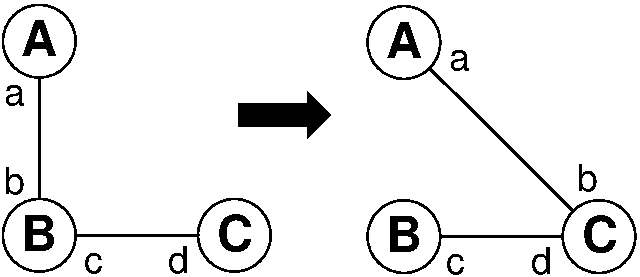
\includegraphics[width=0.8\columnwidth]{img/DelegCase1.pdf}
        \label{fig:bt:deleg-cases:simple}
        %\caption{Simple Delegation}
      }\\
      \subfloat[][Simultaneous delegation \\ ($\triestosend{A}{a}{B}{e}$ and $\triestosend{B}{b}{C}{c}$)]{
       %\begin{center}
       %\vspace{1ex}
       %$\triestosend{A}{e}{B}{a} \quad \triestosend{B}{b}{C}{c}\qquad$
       %\end{center}
        \centering
        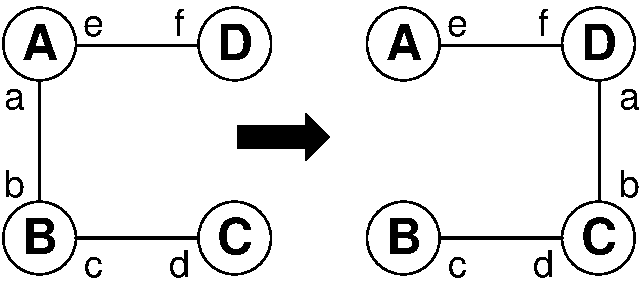
\includegraphics[width=0.9\columnwidth]{img/DelegCase3.pdf}
        \label{fig:bt:deleg-cases:simultaneous}
      %  \caption{Simultaneous Delegation}
      }
    \end{minipage}
    \hfill
    \begin{minipage}{0.475\textwidth}
      \subfloat[][Entangled delegation \\
      ($\triestosend{A}{e}{B}{a}$ and $\triestosend{B}{b}{C}{c}$)]{
       %   \begin{center}
       %     $\triestosend{A}{e}{B}{a} \quad \triestosend{B}{b}{C}{c}\qquad$
       %   \end{center}
        \centering
          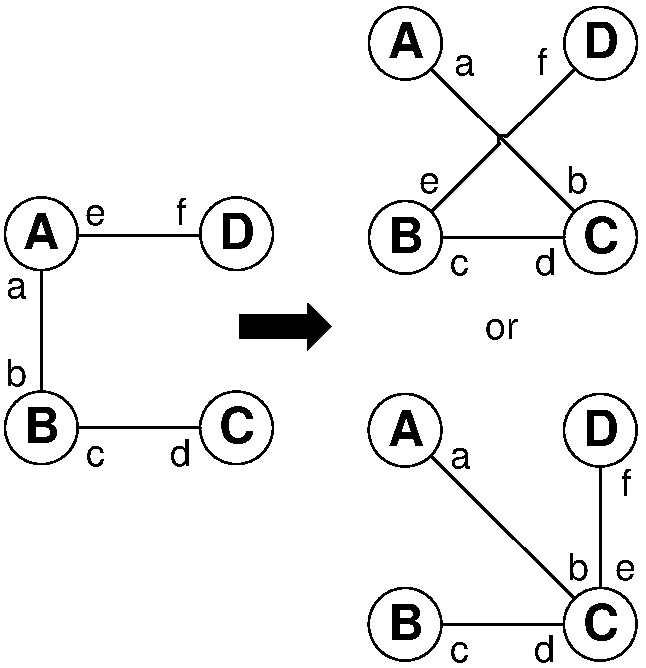
\includegraphics[width=0.8\columnwidth]{img/DelegCase2.pdf}
          \label{fig:bt:deleg-cases:entangled}
          %\caption{Entangled Delegation}
        }
    \end{minipage}
    \caption{Cases of Distributed Delegation}
    \label{fig:bt:deleg-cases}
  \end{figure}



  \mypar{Lost messages.}
  A key issue with distributed delegation is the issue of \emph{lost messages}.
  Consider Figure~\ref{fig:bt:deleg-cases:simple}: process $A$ is connected to
  process $B$ by a channel with endpoints $a$ and $b$, and process $B$ is
  connected to process $C$ by a channel with endpoints $c$ and $d$. Now, suppose
  process $B$ wishes to send endpoint $b$ to process $C$ over endpoint $c$,
  written $\triestosend{B}{b}{C}{c}$.

  If endpoint $b$ has an output type (for example, $\gvout{\intty}{\gvend}$), then the
  delegation can be done straightforwardly: it is possible to transfer all
  messages in the buffer associated with $b$ along with the endpoint, in the
  knowledge that no further messages will arrive while the delegation is in
  progress. However, if endpoint $b$ has an input type (for example,
  $\gvin{\intty}{\gvend}$), then the picture is more complicated, since $A$ can
  send a message over $a$---but it may be the case that $A$ still believes that
  $b$ is located at $B$ when in fact $b$ is located at $C$. Messages delivered
  to the wrong participant in this manner are called \emph{lost messages}.

  \mypar{Simultaneous and entangled delegation.}
  We have so far only considered the simplest case of delegation, where a single
  channel delegation takes place at a time.
  Figure~\ref{fig:bt:deleg-cases:simultaneous} shows \emph{simultaneous}
  delegation, where both endpoints of a channel are delegated at once.

  Furthermore, Figure~\ref{fig:bt:deleg-cases:entangled} shows \emph{entangled}
  delegation, where an endpoint is being sent over an endpoint where the
  receiving peer endpoint is also being delegated. In the case of
  Figure~\ref{fig:bt:deleg-cases}, we have that $A$ is sending endpoint $e$ over
  $a$, to be received by $B$ using endpoint $b$; but at the same time, $B$ is
  sending $b$ to $C$ over endpoint $c$. Due to a lack of causality, we have two
  potential outcomes: either $\triestosend{A}{e}{B}{a}$ happens before
  $\triestosend{B}{b}{C}{c}$, leading to the topology at the top of the figure,
  or $\triestosend{B}{b}{C}{c}$ happens before $\triestosend{A}{e}{B}{a}$,
  leading to the topology at the bottom of the figure.

  A correct distributed delegation algorithm must be able to avoid lost messages
  in all three cases.

  \subsubsection{Na\"ive approaches}
  The simplest solution to avoiding the issues posed by distributed delegation
  is to give up locality, and locate all buffers at some central locations. All
  send and receive operations would then need to contact the central registry;
  as queues do not move, delegation is as simple as passing names. Such an
  approach excels in its simplicity, but requiring a remote call for every
  receive operation is incredibly detrimental to performance, and introduces a
  single point of failure.

  A second na\"ive approach is indefinite redirection: given
  $\triestosend{B}{b}{C}{c}$ in the first scenario, $B$ would be indefinitely
  responsible for forwarding any messages destined for endpoint $b$. Such an
  approach makes delegation somewhat more straightforward since lost messages
  can no longer occur, while also retaining locality of message queues. It is,
  however, impractical since $B$ must remain online indefinitely. Furthermore,
  subsequent delegations can result in long forwarding chains.

  \subsubsection{Distributed Delegation Algorithms}
  The problem of distributed delegation was first studied by Hu et
  al.~\cite{HuYH08:session-java}, who provided the first distributed
  implementation of binary session types as an extension to Java. In order to
  implement distributed delegation without resorting to centralising the
  buffers or using indefinite redirection, Hu et al.\ introduce two algorithms
  for distributed delegation. These two algorithms ensure that the session types
  are respected by ensuring that lost messages are delivered before a session
  progresses.

  The first algorithm is the \emph{resending protocol}. The idea behind the
  resending protocol is to use session type introspection at runtime in order to
  calculate the set of lost messages, which can then be resent from a cache. The
  second algorithm is the \emph{forwarding protocol}, which follows a similar
  pattern as the indefinite redirection approach by forwarding all lost
  messages. Unlike indefinite redirection, however, the forwarding needs only to
  take place until the delegation step has completed, signalled by an
  acknowledgement message.

  \subsubsection{Continuation-passing Approaches}

  \mypar{Linear $\pi$-calculus.}
  Session types were originally studied in the context of specialised process
  calculi extended with session constructs~\cite{Honda93:dyadic,
  HondaVK98:primitives}. Later work by Kobayashi~\cite{Kobayashi02:type-systems}
  sketches a translation into a more canonical calculus: the linear
  $\pi$-calculus~\cite{KobayashiPT99:linear-pi}. The linear $\pi$-calculus is a
  variation of the typed $\pi$-calculus which assigns each name a \emph{payload type},
  \emph{polarity}, and \emph{multiplicity}. The payload type is the type of
  value which can be transmitted over the name. The \emph{polarity} restricts
  whether a name can be used to send or receive a name. Finally, the
  \emph{multiplicity} states the number of times that a name can be used. For
  our purposes, we consider names which must be used precisely once.

  Kobayashi's translation relies crucially on variant types and continuation-passing
  style~\cite{SussmanS98:scheme}. The translation was significantly
  expanded upon by Dardha et al.~\cite{DardhaGS17:revisited}, who proved that
  it was type- and semantics-preserving, and showed that the
  techniques explored by the translation could be adapted to support extensions
  such as subtyping and polymorphism.

  \mypar{Lightweight session types in Scala.}
  Scalas \& Yoshida~\cite{ScalasY16:session-scala} make use of the
  continuation-passing encoding in order to implement \texttt{lchannels}, a
  session type library for Scala.
  %
  To represent the linear $\pi$-calculus in a programming language, Scalas \&
  Yoshida define two types: \verb+In[A]+, a one-shot channel which can be used
  to receive a value of type \verb+A+, and \verb+Out[A]+, a one-shot channel
  which can be used to send a value of type \verb+A+.
  %
  Linearity is checked at runtime. The library provides a
  local implementation using Scala's
  implementations~\cite{HallerPMKKJ:futures} of futures and
  promises~\cite{LiskovS88:promises}. More specifically, the \verb+Out[A]+ type
  is implemented using a \verb+Promise[A]+, and the \verb+In[A]+ type is
  implemented using a \verb+Future[A]+.

  \mypar{Distributed \texttt{lchannels}.}
  In addition to the local implementation, \texttt{lchannels} supports distribution
  by using the Akka actor library~\cite{akka} as an underlying transport.
  The \verb+Out[A]+ type is straightforwardly implemented as a wrapper around an
  actor reference \verb+ActorRef[A]+, which can be used to send a message of
  type \verb+A+ to an actor. However, since it is by design not possible to
  transmit the receive capability of an actor (and mirroring the difficulties
  with distributed delegation), there is no direct analogue to the \verb+In[A]+
  type in the actor setting.

  Their approach to serialising the \verb+In[A]+ type in the actor setting, and
  thus implementing distributed delegation, is to implement a \verb+Dispatcher+
  actor, the reference to which is shared between the \verb+In[A]+ and
  \verb+Out[A]+ channels. Sending along an \verb+Out[A]+ sends a value to the
  dispatcher, and receiving from a \verb+In[A]+ sends a request to the
  dispatcher to retrieve a value when it arrives. Since the buffer of a delegated
  receive endpoint is not tied the receive endpoint, there is no scope for
  lost messages and as such no distributed delegation algorithm is required.
  The approach is therefore a refinement on having a centralised buffer, the
  differences being that a dispatcher actor can be spawned at the last-known
  location of the receiver for efficiency, and that a dispatcher actor handles a
  single message at a time rather than a sequence of messages.

  \mypar{Multiparty extension.}
  Scalas et al.~\cite{ScalasDHY17:mpst-decomposition} extend the
  continuation-passing encoding to the multiparty setting, by showing how a
  \emph{multiparty} session calculus can be encoded in the linear
  $\pi$-calculus, and show that the translation is type- and
  semantics-preserving.

  By virtue of the translation into the linear $\pi$-calculus, Scalas et al.\
  show the first implementation of \emph{multiparty} delegation by leveraging
  the infrastructure already provided by \texttt{lchannels}. In contrast to
  binary session types, no explicit distributed delegation algorithms exist for
  multiparty session types due to the co-ordination needed between different
  parties. Indeed, such an algorithm would likely be complex.

  \subsection{Behavioural types for Actor Systems}\label{sec:bt:actor-types}
  The \emph{actor model} was introduced as a formalism for artificial
  intelligence by Hewitt et al.~\cite{HewittBS73:actors}. An actor is an entity with a
  unique identifier which upon receiving a message can perform
  three actions: it can send a finite set of messages to other actors; spawn a
  finite set of new actors; and change how it reacts to a new message being
  received.

  \begin{figure}[t]
\centering
\subfloat[Channel\label{fig:bt:channels-vs-mailboxes:a}]{
  \centering
  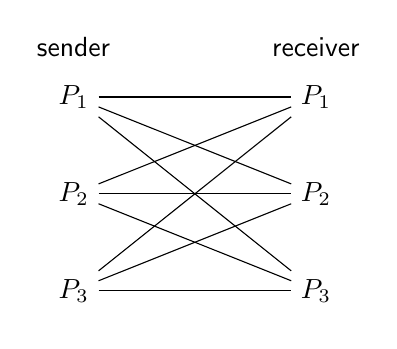
\begin{tikzpicture}

    \matrix (m) [matrix of math nodes,row sep=2em,column sep=7em,minimum
    width=1em,ampersand replacement=\&]
    {
       P_1 \& P_1 \\
       P_2 \& P_2 \\
       P_3 \& P_3 \\
    };
    \path
      (m-1-1) edge (m-1-2)
              edge (m-2-2)
              edge (m-3-2)
      (m-2-1) edge (m-1-2)
              edge (m-2-2)
              edge (m-3-2)
      (m-3-1) edge (m-1-2)
              edge (m-2-2)
              edge (m-3-2);

    %% \tikzset{dotted/.style={draw=black!50!white, line width=0.5pt,
    %%                         dash pattern=on 2pt off 2pt,
    %%                         inner sep=0mm, rectangle, rounded corners}};

    \node (sender) [fit = (m-1-1) (m-3-1)] {};
    \node at (sender.north) [above] {\textsf{sender}};

    \node (receiver) [fit = (m-1-2) (m-3-2)] {};
    \node at (receiver.north) [above] {\textsf{receiver}};

  \end{tikzpicture}
}
~
\subfloat[Mailbox\label{fig:bt:channels-vs-mailboxes:b}]{
  \centering
  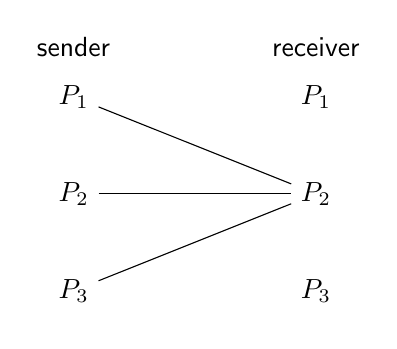
\begin{tikzpicture}
    \matrix (m) [matrix of math nodes,row sep=2em,column sep=7em,minimum
    width=1em,ampersand replacement=\&]
    {
       P_1 \& P_1 \\
       P_2 \& P_2 \\
       P_3 \& P_3 \\
    };
    \path
      (m-1-1) edge (m-2-2)
      (m-2-1) edge (m-2-2)
      (m-3-1) edge (m-2-2);

    \node (sender) [fit = (m-1-1) (m-3-1)] {};
    \node at (sender.north) [above] {\textsf{sender}};

    \node (receiver) [fit = (m-1-2) (m-3-2)] {};
    \node at (receiver.north) [above] {\textsf{receiver}};

  \end{tikzpicture}
}

\caption{Channel-style vs.\ actor-style communication}
\label{fig:bt:channels-vs-mailboxes}
\end{figure}


  Agha~\cite{Agha90:actors} was first to investigate the actor model as a formalism
  for distributed systems. The actor model is particularly appealing since
  process IDs can be used to \emph{send} messages, but the capability to
  \emph{receive} messages is associated uniquely with an actor. In turn, this
  restriction sidesteps the issues described in
  Section~\ref{sec:bt:distrib-deleg}.
  This asymmetry is captured by Figure~\ref{fig:bt:channels-vs-mailboxes} (Figure
  as shown by Fowler et al.~\cite{FowlerLW17:mm}). Figure~\ref{fig:bt:channels-vs-mailboxes:a}
  shows the communication patterns allowed by three process $P_1$, $P_2$, and
  $P_3$, over a channel: given that each process has access to the channel,
  each process can use the channel to send a message to any of the other
  processes. Figure~\ref{fig:bt:channels-vs-mailboxes:b} shows the communication
  patterns associated with process $P_2$ as an actor process: given the process
  ID of $P_2$, all processes can send $P_2$ a message, but only $P_2$ can
  receive messages.

  \mypar{The Challenges of Typed Mailboxes}
  Actor communication is asynchronous. When implementing actors, an
  implementation technique is to associate each process with an incoming message
  queue, or \emph{mailbox}. While adding types to channels is entirely
  straightforward, adding types to mailboxes is substantially more challenging.

  Most implementations of actor-like communication, such as processes in
  Erlang~\cite{Armstrong10:erlang} or the native actor libraries for
  Scala~\cite{HallerO09:actors}, provide untyped mailboxes.
  %
  Typed mailboxes were first investigated by~He et al.~\cite{HeWT14:actors}, who
  introduced a typed extension of Akka, called TAkka. The authors highlighted
  the \emph{type pollution} problem, aparticular challenge with typed mailboxes
  arising due to the coarser granularity of typing.

  \begin{figure}[t]
    \centering
    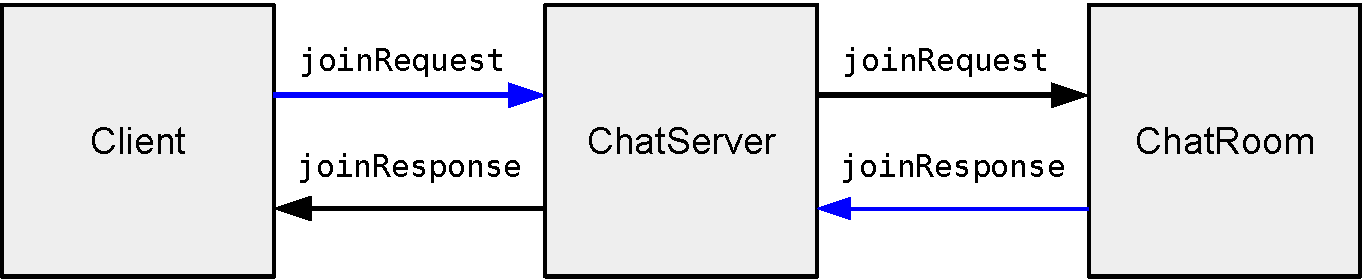
\includegraphics[width=0.75\textwidth]{img/type-pollution-example.pdf}
    \caption{Type Pollution}
    \label{fig:bt:type-pollution}
  \end{figure}

  To demonstrate this,
  consider the scenario shown in Figure~\ref{fig:bt:type-pollution}. A client
  wishes to connect to a chat room, modelled by a \lstinline+ChatRoom+ actor. It
  firstly sends a \lstinline+joinRequest+ message to the \lstinline+ChatServer+
  actor, which forwards the request to the appropriate \lstinline+ChatRoom+
  actor. The \lstinline+ChatRoom+ actor responds with a \lstinline+joinResponse+
  message, which is then forwarded to the client. We can assign the following
  mailbox types:


  \begin{itemize}
    \item \lstinline|Client : ActorRef(joinResponse)|
    \item \lstinline|ChatServer : ActorRef(joinRequest + joinResponse)|
    \item \lstinline|ChatRoom : ActorRef(joinRequest)|
  \end{itemize}

  Note in particular that the \lstinline+ChatServer+ must be able to handle both
  the \lstinline+joinRequest+ \emph{and} the \lstinline+joinResponse+ messages.
  Na\"ively implemented, this would result in a complete loss of modularity:
  each actor would be aware of \emph{every} message which could be received by
  every other actor, and worse, would need to use the exact same sum injection.
  Any small changes would make the program ill-typed.

  He et al.~\cite{HeWT14:actors} address type pollution by making use of subtyping, making
  actor references contravariant in their message type. Using a similar
  approach, the widely-adopted Akka framework~\cite{akka} has recently
  transitioned to typed actor references; the first major actor framework to do so.

  Fowler et al.~\cite{FowlerLW17:mm} study typed actors formally, and formally investigate
  type- and semantics-preserving translations between the two communication
  models. In particular, the type pollution problem means that in order to
  translate from typed channels into typed actors, one must either assign the
  same type to every channel in the system, or use a synchronisation mechanism
  such as futures.

  \mypar{A na\"ive behavioural type system for mailboxes.}
  As---unlike channels---mailboxes are unidirectional, the na\"ive extension is
  to generalise an actor's mailbox type to receiving a \emph{sequence} of types.
  Letting $A, B$ range over types, $V$ range over values, and $M$ range over
  terms, we might envisage actor references of type $\pid{\seq{A}}$ and the
  following two communication constructs:

  \begin{mathpar}
    \inferrule
      [TA-Receive]
      { }
      { \cdot \mid A \cdot \seq{A} \triangleright \calcwd{receive} : A \triangleleft \seq{A} }

    \inferrule
      [TA-Send]
      { \Gamma_1 \vdash V : A \\ \Gamma_2 \vdash W : \pid{A \cdot \seq{A}} }
      { \Gamma_1, \Gamma_2 \mid \seq{B} \triangleright \calcwd{send} \: M : \pid{A} \triangleleft \seq{B} }
  \end{mathpar}

  The $\Gamma \mid \seq{A} \triangleright M : B \triangleleft \seq{A}'$
  judgement can be read ``Under typing environment $\Gamma$, with the ability to
  receive a sequence of values with types $\seq{A}$, term $M$ has type $B$, and the
  remainder of the program has the ability to receive a sequence of values with
  type $\seq{A}'$. As values are pure, the value typing judgement $\Gamma \vdash
  V : A$ states that under type environment $\Gamma$, value $V$ has type $A$.

  Given the ability to receive values of types $A \cdot \seq{A}$, rule \textsc{TA-Receive}
  assigns $\calcwd{receive}$ type $A$, and allows $\seq{A}$ to be received in
  the remainder of the program. Correspondingly, rule \textsc{TA-Send} assigns
  term $\calcwd{send} \: V \: W$ type $\pid{A}$ if value $V$ has type $A$ and
  value $W$ is a process ID with type $\pid{A \cdot \seq{A}}$. Sending a message
  does not affect the types of value that the sender can receive.
  This formulation of a calculus with effectful operations with pre- and
  post-conditions is reminiscent of a parameterised
  monad~\cite{Atkey09:parameterised}.

  In order to make such a system sound, since $\calcwd{send}$ changes the type
  of a process ID, we need a linear type system. Unfortunately, such a system is
  far too restrictive to use in practice: as a gauge, there is no obvious
  translation from a standard channel-based session calculus into the above
  behavioural type system.

  In the remainder of this section, we survey various approaches to assigning
  behavioural types to actor-like systems.

  \subsubsection{Featherweight Erlang}
  Erlang~\cite{Armstrong10:erlang} is a dynamically-typed concurrent functional
  programming language, originally designed for telecommunications applications.
  Erlang was designed to allow developers to write applications with strong
  reliability guarantees, fostering a development style with share-nothing
  semantics and explicit message passing.
  %
  Although the developers did not
  explicitly base their design on the actor model~\cite{erlang-not-actor}, the
  language provides addressable processes with an incoming message queue, so
  follows similar principles; indeed,~Agha et
  al.~\cite{AghaMST97:foundation-actor} describe Erlang as ``essentially
  an actor language''.

  Erlang supports a \emph{selective receive} construct, which supports pattern
  matching syntax to await messages of a particular structure.
  %
  Mostrous \& Vasconcelos~\cite{MostrousV11:session-erlang} describe a
  behaviourally-typed process calculus which allows a form of binary session
  typing. The key idea is to emulate session channels using two key ingredients:
  selective receive, and a mechanism to generate unique references. Unique
  references can then be used as a proxy for a session channel endpoint; a
  technique known as \emph{correlation sets}~\cite{Viroli04a:correlation}. By
  combining selective receive and unique references with a behavioural typing
  discipline, it becomes possible to specify and check binary session protocols.

  Their approach has not been implemented. A key drawback is that the approach
  forbids delegation, so the communication topology remains static. It would be
  interesting to implement the system and see whether it scales to larger
  examples, and whether the correlation sets approach could be used to implement
  multiparty session types. Due to the issues identified in
  Section~\ref{sec:bt:distrib-deleg}, it is likely that supporting
  delegation would be challenging.

  \subsubsection{Runtime Monitoring}
  In Section~\ref{sec:bt:mpst}, we described how the correspondence between
  multiparty session types and communicating finite state automata has given
  rise to implementations which allow conformance to multiparty session types to
  be checked at runtime.

  \begin{figure}[t]

    \subfloat[fig:bt:mpsa1][Standard MPST Monitoring]{
      \label{fig:bt:mpsa1}
      \centering
      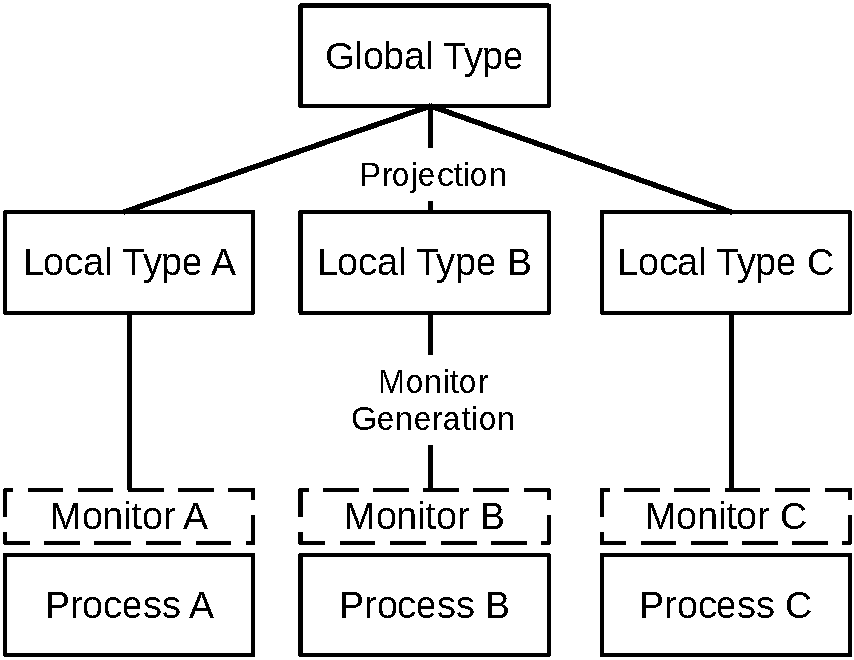
\includegraphics[width=0.45\textwidth]{img/mpst-diag.pdf}
    }
    %
    \hfill
    %
    \subfloat[fig:bt:mpsa2][Multiparty Session Actors]{
      \label{fig:bt:mpsa2}
      \centering
      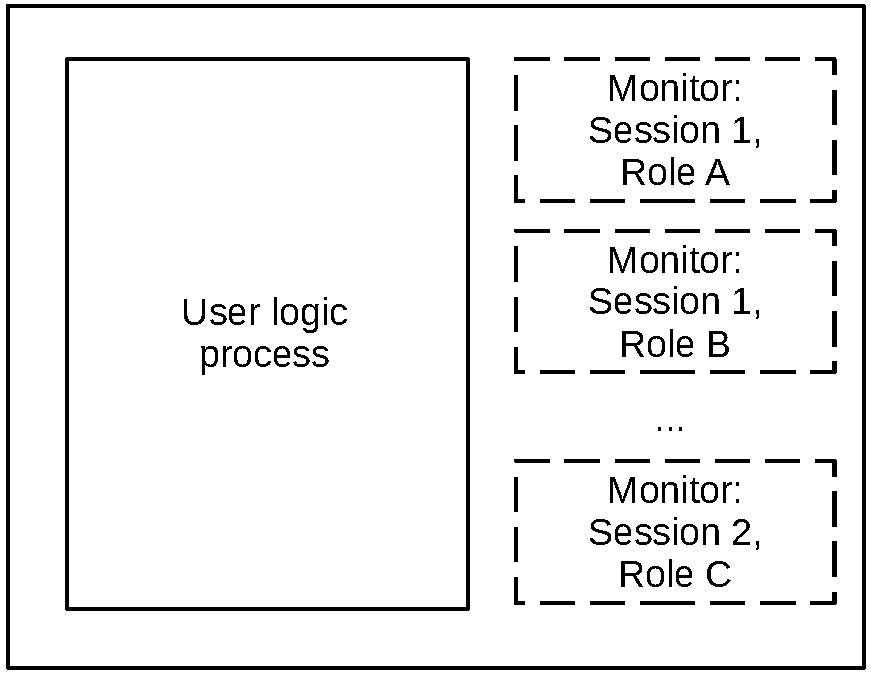
\includegraphics[width=0.4\textwidth]{img/mpsa-diag.pdf}
    }
    \caption{Monitored processes vs. multiparty session actors}
    \label{fig:bt:mpst-actor}
  \end{figure}


  Neykova \& Yoshida~\cite{NeykovaY16:sactor} implemented a Python framework for
  actor-style communication.
  In the `classic' approach to monitoring processes using multiparty session
  types (Figure~\ref{fig:bt:mpsa1}), each process implements a single role in a
  protocol, with communication mediated by a monitor generated from a local
  type.
  In the multiparty session actors approach,
  The key differences over the `classic' approach (Figure~\ref{fig:bt:mpsa2}),
  each actor may play \emph{multiple} roles in \emph{multiple} sessions at a
  time; is driven by incoming messages; and that a message received in one
  session may trigger communication in another.

  Neykova \& Yoshida use the Celery~\cite{celery} framework to build their
  library. Python is an imperative language which does not support native
  concurrency, nor enforce actor-style fault isolation.
  Fowler~\cite{Fowler16:actors} implements Neykova \& Yoshida's conceptual
  framework in Erlang, and introduces dynamism in the communication topologies,
  along with some rudimentary failure handling
  mechanisms, using subsessions, as introduced by Demangeon \&
  Honda~\cite{DemangeonH12:subsessions}. Failure handling is crucial in the
  distributed setting, and we discuss it further in
  Section~\ref{sec:bt:failure-handling}.

  \subsubsection{Parameterised Actor Systems}
  \todo{Summarise~\cite{CharalambidesDA16:param-actors}}

  \subsubsection{Types for Actor Progress}
  \todo{Summarise~\cite{CharalambidesPA19:actor-progress}}


  \subsubsection{Mailbox Types}
  Our na\"ive behavioural type system from Section~\ref{sec:bt:actor-types} was too
  restrictive as it required that messages were received in a particular order,
  which in turn necessitated that a reference used to send messages to an actor
  was linear.

  de'Liguoro \& Padovani~\cite{deLiguoroP18:mailbox} instead propose the \emph{mailbox calculus}
  and a mailbox typing system for \emph{unordered} interactions.

  The mailbox calculus is similar to the asynchronous $\pi$-calculus in that
  message sends do not have a continuation. Whereas actor-style calculi tend to
  associate a process with a \emph{single} mailbox, the mailbox calculus allows
  each process to be associated with \emph{multiple} mailboxes, and supports
  nondeterministically selective receiving messages between them.
  The authors then propose a behavioural typing system which, via a
  dependency graph, ensures that processes do not fail due to unexpected
  messages; do not deadlock; and (for certain processes) do not allow
  unprocessed messages.

  The behavioural type system for the mailbox typing system is appealing in
  several respects. First, as shown by de'Liguoro \& Padovani, it is expressive
  enough to encode real communication patterns, as shown by the encodings of
  several applications from the Savina benchmark suite~\cite{ImamS14:savina}. Second, due
  to the receive-only nature of mailboxes, it does not suffer from the
  distributed delegation issues described in Section~\ref{sec:bt:distrib-deleg}.
  Third, even without considering message ordering, the type system ensures
  useful
  safety properties.

  \subsection{Failure handling}\label{sec:bt:failure-handling}

  A key difference between the concurrent and distributed settings is the
  ability to handle failures. Whereas in the concurrent setting it is reasonable
  to expect that all participants will be online for the duration of a session,
  and that all messages will be reliably delivered, this is not the case in the
  distributed setting.

  In this section, we describe various proposals towards extending session types
  and communication-centric behavioural typing disciplines with support for
  failure handling.

  \begin{figure}[t]
    \centering
    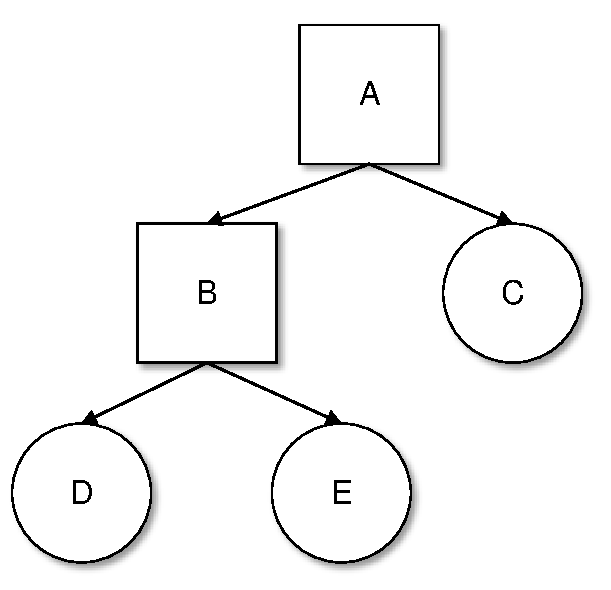
\includegraphics[width=0.3\textwidth]{img/SupervisionTree.pdf}
    \caption{Supervision hierarchy}
    \label{fig:bt:supervision}
  \end{figure}

  \subsubsection{Erlang}
  In distributed systems, failure is inevitable. Key to Erlang's success is that
  it was  designed with failure handling as a key concern. In Erlang, processes
  are arranged in supervision hierarchies~\cite{Armstrong03:thesis} (see
  Figure~\ref{fig:bt:supervision}). In this example, if process \texttt{B}
  encounters an unrecoverable error, it should be designed to crash; its
  supervisor process \texttt{D} will then be notified of the failure, and can
  restart the process.

  Fowler~\cite{Fowler16:actors} implements Neykova \& Yoshida's session actor
  framework~\cite{NeykovaY16:sactor} in Erlang. If a monitor rejects a message,
  this is treated as an unrecoverable failure, and the process is terminated.
  If a process crashes, a reachability analysis is used to detect whether the
  process is needed in the remainder of each session in which it is involved; if
  the process is not involved, then the sessions can continue. The author also
  advocates splitting a session into multiple possibly-failing subsessions in
  order to localise failures, and presents a simple exception handling
  construct. The approach is not formalised.

  Neykova \& Yoshida~\cite{NeykovaY17:let-it-recover} propose a more
  sophisticated mechanism which allows safe recovery for various supervision
  strategies, rather than treating a crash where a participant is required in
  the remainder of the session as unrecoverable. The authors define an algorithm
  to statically determine the dependencies induced by a protocol, which are
  stored in a global recovery table. The global recovery table can be used to
  recover from partial failures in the system by triggering the re-sending of
  required messages upon detection of a failure. The approach is formalised, and
  the authors show safety and transparency properties. Furthermore, the
  performance of the approach is evaluated empirically to show that protocol
  recovery outperforms the na\"ive recovery strategies.

  \subsubsection{Availability and crash handling.}

  \mypar{Typing availability.}
  Choreographic programming~\cite{CarboneM13:df-design} allows a developer to
  specify deadlock-free protocols at a global level, and allows code generation
  for each participant. L\'opez et al.~\cite{LopezNN16:availability} describe an
  approach to choreographic programming for cyber-physical systems such as
  sensor networks. They introduce the \emph{Global Quality Calculus}, an
  extension of the Global Calculus~\cite{CarboneM13:df-design} to include
  broadcast and gathering constructs. Each communication action is annotated
  with \emph{quality predicates}, which record the number of nodes which must be
  available for a communication to occur. Each thread is annotated with
  \emph{progress capabilities}, which define the preconditions required for a
  thread to evaluate, and the capabilities after a communication has occurred.
  The calculus supports graceful degradation of the system, and the authors
  provide a behavioural typing discipline to ensure that the calculus enjoys
  progress.

  \mypar{Protocol types.}
  Chen et al.~\cite{ChenVBZE16:failure-handling} introduce \emph{protocol
  types}, a type disipline inspired by multiparty session types. Communication
  actions are annotated by failure conditions that might be raised as a result
  of a message, and failures can be handled by performing a set of interactions
  described in an associated failure handling block. Analogously to projecting a
  global type into a local type, a protocol type is \emph{transformed} into
  local types which include explicit synchronisation points in order to ensure
  that all affected participants are notified when a failure takes place.

  \mypar{Link failures.}
  Adameit et al.~\cite{AdameitPN17:link-failures} describe a multiparty session
  calculus extended with \emph{optional blocks}. An optional block describes a
  portion of the protocol to be run as a possibly-failing
  subsession~\cite{DemangeonH12:subsessions}, along with a default value to be
  used should the subsession fail. The authors illustrate the technique on the
  rotating coordinators algorithm~\cite{Tel00:dist-algorithms}.


  \mypar{Broadcast.}
  Kouzapas et al.~\cite{KouzapasGVG19:async-broadcast} describe a session
  process calculus designed for broadcast communication, where a single sender
  can send messages to multiple
  receivers. A key distinguishing feature is that their calculus allows for
  \emph{unreliable} interactions, where messages can be lost during
  transmissions. The authors show that their approach is expressive enough to
  encode the failure-aware Paxos~\cite{Lamport98:paxos} protocol for distributed
  consensus.

  \mypar{Crash handling via a coordinator process.}
  Viering et al.~\cite{VieringCEHZ18:crash-handling} describe a process calculus
  and multiparty session typing discipline to handle \emph{crash failures} in
  distributed systems. They assume reliable communication and a robust
  coordinator process, as well as reliable failure detection, but due to
  asynchrony there is no total ordering on the messages transmitted in the
  system.
%
  Although the assumptions of a robust co-ordinator process and reliable failure
  detection sound strong, robust processes are implemented in practice using
  techniques such as redundant services and consensus prototcols; an example is
  the popular Apache ZooKeeper project~\cite{JunqueiraR13:zookeeper}. Reliable
  failure detection can be approximated by timeouts, and signalling that a
  process should crash if it is suspected of having failed.

  The authors extend multiparty session types with a
  \mkwd{try}-\mkwd{handler} block which can be arbitrarily nested; each failure
  handler specifies a set of failed roles (i.e., roles provided by processes
  which have crashed), and the system is guaranteed by the type system to be in
  a consistent state at the end of a \mkwd{try}-\mkwd{handle} block.

  \subsubsection{Interactional exceptions and global escape.}
  Carbone et al.~\cite{CarboneHY08:exceptions} were first to consider extending
  an asynchronous session-typed process calculus with an exception handling
  construct. Their key idea is to introduce a service channel type which includes an
  \emph{exception handling clause} describing an interaction pattern to be
  invoked should an exception arise. As an example, this pattern makes it
  possible to abort an otherwise infinite interaction. The approach also
  supports nested exceptions. To guarantee liveness in the presence of nested
  exceptions, message queues are annotated with exception levels; when an
  exception occurs, the system guarantees liveness by propagating an exception
  message through the system. Although the seminal work on considering session
  types with exceptions, perhaps due in part to its complexity, the system has
  not been implemented.

  Capecchi et al.~\cite{CapecchiGY16:global-escape} propose a similar approach
  for multiparty session types. Instead of providing services with an exception
  handling clause, they include an explicit $\mkwd{try}-\mkwd{catch}$ block
  along with labelled queue levels; care is required in order to propagate the
  exception to all affected parties.

  \subsubsection{Affine sessions.}

  Linear type systems forbid the properties of weakening (computationally,
  allowing a resource to be discarded) and contraction (computationally,
  allowing a resource to be duplicated).  Taken together, these two restrictions
  on structural rules ensure that a linear resource must be used precisely once.
  Unfortunately, in the presence of failure, a linear type system is too strong
  as one party may crash and therefore not be able to complete their part of the
  protocol.

  \mypar{Affine type systems.}
  One possible solution is to use an \emph{affine} type system. An affine type
  system forbids contraction, but allows weakening,
  meaning that session endpoints can be discarded.
%
  The main problem with using an affine type system is that it is possible to
  write a program where one party does not complete their role in the
  communication protocol, and the other party is blocked indefinitely.
  Furthermore, a developer does not get any feedback if they \emph{accidentally}
  forget to implement part of a protocol.

  \mypar{Explicit cancellation.}
  Mostrous \& Vasconcelos~\cite{MostrousV18:affine} introduce a session-typed
  process calculus with \emph{explicit cancellation} to denote an endpoint which
  can no longer be used for communication. Attempting to send or receive along
  an endpoint whose peer is cancelled results in an exception being thrown; the
  exception can be caught using an exception handler process.

  Fowler et al.~\cite{FowlerLMD19:stwt} build upon the work of Mostrous \&
  Vasconcelos by introducing Exceptional GV: an extension of the GV
  session-typed $\lambda$-calculus with explicit cancellations, exception
  handlers, and asynchrony. The exception handling construct in EGV is
  compositional and allows arbitrary nesting of exception handlers, whereas the
  exception handler process in the work of Mostrous \& Vasconcelos scopes only
  over a single communication action. Furthermore, Fowler et al.\ provide an
  implementation of the technique in the Links programming
  language~\cite{CooperLWY06:links}, in turn providing the first application of
  session types to web programming.

  \mypar{Adjoint logic.}
  Pruiksma \& Pfenning~\cite{PruiksmaP19:mp-adjoint} provide a logical grounding
  for cancellation (as well as multicast and replication) by providing a
  message-passing interpretation of adjoint logic~\cite{PruiksmaCPR18:adjoint}.
  The key computational idea is to interpret the logical cut rule as the process
  $S \leftarrow (\nu x) P; Q$, where $S$ is a possibly-empty set of channels
  provided by process $P$, $x$ is the internal name of a channel used by $P$;
  and $Q$ is a continuation process. If $S$ is a singleton set, then the normal
  semantics are used; if $S$ is the empty set, then $x$ is cancelled; and if $S$
  is a set containing multiple names, then $x$ is used for multicast.

  \section{Future Directions}\label{sec:bt:future}
  Although there has been much work on behavioural typing, including much
  pertaining to the distributed session, the field remains ripe for future work.
  A key theme is putting theory into practice, in particular developing ideas
  conceived for process calculi into concrete language designs and
  implementations. In this section, we propose four concrete directions: formal
  models of distributed delegation algorithms; a programming language based on
  the Mailbox Calculus; an implementation of exception handling in the
  multiparty setting; and behavioural types for future combinator libraries.

  \subsection{Formal models of distributed delegation algorithms}
  To handle the intricacies of session delegation in the presence of
  distribution and asynchrony, Hu et al.~\cite{HuYH08:session-java} developed
  distributed delegation algorithms. These algorithms were presented by example
  and proved informally. It would be interesting to implement the algorithms in
  a tool such as TLA+~\cite{Lamport2002:tlaplus} in order to provide a reference
  algorithmic presentation, and to machine-check their correctness.

  Additionally, it would be interesting to perform a performance comparison
  between the explicit distributed delegation algorithms presented by Hu et
  al.~\cite{HuYH08:session-java} and the continuation-passing approach presented
  by Scalas \& Yoshida~\cite{ScalasY16:session-scala}.

  \subsection{A language based on the Mailbox Calculus}
  The Mailbox Calculus, proposed by de'Liguoro \&
  Padovani~\cite{deLiguoroP18:mailbox}, is a particularly
  appealing proposal for a distribution-friendly behavioural type system.
  However, process calculi are useful for modelling the \emph{state} of a
  system, but it is difficult to immediately see the \emph{program} one would
  write in order to arrive at such a state. Consequently, it would be
  interesting to consider a concrete language design for the mailbox calculus.
  Furthermore, Padovani~\cite{Padovani18:mc2} has implemented a typechecker for
  the mailbox calculus, but not a runtime system.

  It would be interesting, after a concrete language design, to implement a
  concurrent language runtime, perhaps by compilation to the BEAM virtual
  machine used by Erlang.

  \subsection{Implementing exception handling for multiparty session types}
  While Fowler et al.~\cite{FowlerLMD19:stwt} proposed the first full design and
  implementation of exception handling in a linearly-typed functional
  programming language with session types, based on the work of Mostrous and
  Vasconcelos~\cite{MostrousV18:affine}, their work only handles the binary setting. An
  implementation of multiparty session types with exceptions is still an open
  problem. A key prerequisite is to firstly develop a language design
  incorporating multiparty session types, perhaps extending the functional GV
  calculus~\cite{Wadler14:prop-sessions,LindleyM15:semantics}.

  \subsection{Behavioural types for future combinator libraries}
  As touched upon earlier in the chapter, a \emph{future} is a placeholder for a
  value that is in the process of being computed, and are widely-used for a
  variety of potentially-blocking operations such as network calls. Libraries
  such as Finagle~\cite{finagle} provide combinators for sequencing futures and
  handling potential failures, and have seen significant use in industry. In
  particular, Finagle is widely used at Twitter.

  Although futures are widely adopted, they provide weak guarantees. As a simple
  example, it is possible to wait on a function which never terminates, or to
  create an infinite cycle of futures which will never be resolved.
  It would be interesting to see whether behavioural types could be used in
  order to provide guarantees such as deadlock-freedom. Another avenue for
  exploration could be behavioural-type-guided static analysis techniques such
  as those used proposed by Lange et al.~\cite{LangeNTY17:fencing-off-go} for
  the Go programming language~\cite{DonovanK15:go}.

  \section{Conclusion}\label{sec:bt:conclusion}

  Behavioural types allow properties about the runtime behaviour of a program,
  for example conformance to a protocol, to be checked before a program is run.
  While behavioural typing disciplines are well-understood in the concurrent
  setting, the distributed setting poses challenges.

  In this section, we have given an overview of behavioural type disciplines for
  distribution, in particular concentrating on three issues: distributed
  delegation of session-typed channels; behavioural types for
  distribution-friendly paradigms such as the actor model; and behavioural types
  in the presence of failure.

  Although many complementary approaches have been proposed to allow various
  behavioural properties to be checked, a notable gap is a concrete language
  design which could gain widespread adoption. Perhaps the single largest
  research challenge in this area is to distil the right combination of language
  features and type system features which would be flexible enough to use in
  practice, yet also provide helpful static typechecking to rule out more errors
  at compile time.

	%%%%%%%%%%%%%%%%%%%%%%%%%%%%%%%%%%%%%%%%%%%%%%%%%%%%%%%%%%%%%%%%%%%%%%%%%%%%%%%%%%%%%%%%%%%%%%%%%%%%%%%%
	%% For your bibliography, you should use a bibtex .bib file and include it here.
	%% Note that the final reference lists styling might differ because it'll be styled in unified book layout.

	% \biblstarthook{
	%	text inserted here will be printed before the actual list of references, but only if there is at least one reference to %display. Delete this section if you don't need it.
	%}

	% \nocite{*}		%% uncomment if uncited references should be listed in the bibliography.

	%% uncomment and state path to your .bib to use a bibtex file as your bibliography.
	%% NOTE: relative paths don't work in \putbib => During development, you might delete the "\CHAPTERSROOT/chapter\chapterprefix/" part to refer to your bib file. When you're done, please make this path absolute by adding the prefix again.
	%%
	%\putbib[\CHAPTERSROOT/chapter\chapterprefix/bibliography] %
	\putbib[bibliography] %

\end{bibunit}

%% uncomment the \end{document} statement to make this file stand-alone compileable.
\end{document}
